\section{Auswertung}
\label{sec:Auswertung}
Der Versuch wird, wie in \autoref{sec:Durchführung} aufgebaut und durchgeführt.
\subsection{Bestimmung der Weglänge}
\label{subsec:Weglänge}
Im Folgenden wird die mittlere Weglänge bei verschiedenen Temperaturen bestimmt. Dazu wird mit \autoref{eqn:psät} der Sättigungsdampfdruck $p_{s\ddot{a}t}$ bei den gemessenen 
Temperaturen bestimmt. Danach wird $\bar{\omega}$ mit der \autoref{eqn:Weglänge} bestimmt. Alle Werte werden in die \autoref{tab:Weglänge} eingetragen.
\begin{table}[H]
  \centering
  \caption{Gemsesene und bestimmte Werte für die Wellenlänge.}
  \label{tab:Weglänge}
  \sisetup{table-format=2.2}
  \begin{tabular}{S[table-format=3.2] S[table-format=2.3] S[table-format=1.4] S[table-format=4.1]}
  \toprule
  {Temperatur $T / \si{\kelvin}$} & {Sättigungsdampfdruck $p_{s\ddot{a}t} / \si{\milli\bar}$} & {mittlere Weglänge $\bar{\omega} / \si{\centi\meter}$} & {Verhältnis $\frac{a}{\bar{\omega}}$}\\
  \midrule
    296.45   & 0.005 & 0.6241 & 1602.2 \\
    416.15  & 3.669 & 0.0008  & 1265.2 \\
    442.15  & 9.695 & 0.0003  & 3342.9 \\
    452.15  & 13.674 & 0.0002 & 4715.2 \\
  \bottomrule
  \end{tabular}
\end{table}
Das Verhältnis $\frac{a}{\bar{\omega}}$ wird auch in \autoref{tab:Weglänge} eingetregen mit $a = \qty{1}{\centi\meter}$. 
%T =  [296.45 416.15 442.15 452.15]
%psät=  [4.64657855e-03 3.66913288e+00 9.69451481e+00 1.36740660e+01]
%w =  [6.24115136e-01 7.90377480e-04 2.99138230e-04 2.12080298e-04]
%aw =  [1.60226846e+00 1.26521823e+03 3.34293614e+03 4.71519518e+03]
%Ende der Weglänge

\subsection{Integrale und differentielle Energieverteilung}
\label{subsec:Energieverteilung}

Tiefpunkt für $T_1$ bei $\qty{8.25}{\volt}$ und $T_2$ bei $\qty{1.29}{\volt}$.

Anschließend wird aus den Werten mithilfe der Formel
\begin{align*}
  \frac{\Delta I_A}{\Delta U_A} &= \frac{I_{A_{i+1}}-I_{A_i}}{U_{A_{i+1}}-U_{A_i}}\label{eqn:diffquo}
\end{align*}
stückweise die Differenzenquotienten berechnet.
Die differentielle Darstellung der Energieverteilung wird somit in \autoref{fig:plot2} abgebildet.

\begin{figure}[H]
  \centering
  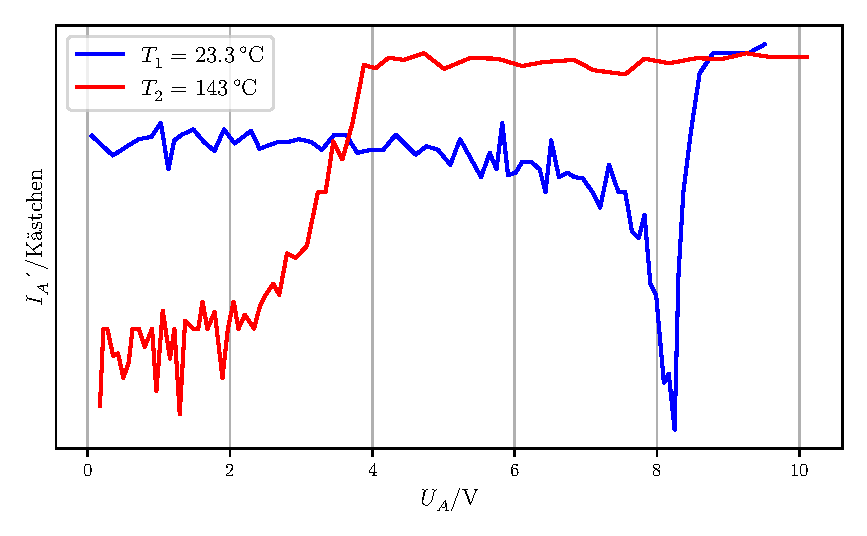
\includegraphics[width=\textwidth]{build/plot2.pdf}
  \caption {Aus der integralen Energieverteilung berechnete differentielle Energieverteilung der Elektronen.}
  \label{fig:plot2}
\end{figure}
Die Tiefpunkte der differentiellen Energieverteilung liegen für $T_1$ bei $\qty{8.25}{\volt}$ und für $T_2$ bei $\qty{1.29}{\volt}$.
Aus der Lage des Tiefpunktes der Kurve von $T_1$ ergibt sich das Kontaktpotential $K$ mit der Beschleunigungsspannung $U_B= \qty{11}{\volt}$
durch Umstellen von \autoref{eqn:UBeff} zu
\begin{align*}
  K_1 &= \qty{11}{\volt}-\qty{8.25}{\volt} &= \qty{2.75}{\volt}.\\
\end{align*}
%Ende der Energieverteilung

\subsection{Franck-Hertz-Kurve} % (fold)
\label{sub:Franck-Hertz-Kurve}
Die Franck-Hertz-Kurve wird bei zwei Temperaturen untersucht und aufgezeichnet (siehe \autoref{fig:plot3} und \autoref{fig:2.jpeg}). 
Die Temperaturen liegen bei $T_3= \qty{169}{\celsius}$ und bei $T_4= \qty{179}{\celsius}$.

\begin{figure}[H]
  \centering
  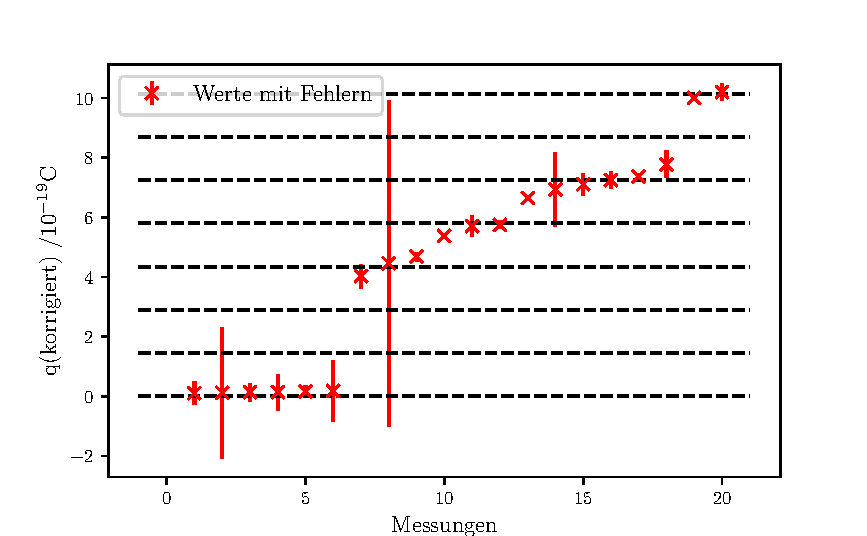
\includegraphics[width=\textwidth]{plot3.pdf}
  \caption{Franck-Hertz-Kurve bei $T_3$ und $T_4$.}
  \label{fig:plot3}
\end{figure}

Im Folgenden wird die Kurve mit der Temperatur $T_3 = \qty{169}{\celsius}$ benutzt, weil diese deutlichere Peaks aufweisen. Zur Vollständigkeit
werden die Werte von der anderen Kurve auch in \autoref{tab:Franck} aufgelistet.

\begin{table}[H]
  \centering
  \caption{Wärmeströme zu verschiedenen Messzeiten.}
  \label{tab:Franck}
  \sisetup{table-format=2.3}
  \begin{tabular}{S S S S S}
    \toprule
    \multicolumn {2}{c}{$T_3 = \qty{169}{\celsius}$}& \multicolumn {2}{c}{$T_4= \qty{179}{\celsius}$}\\
    \cmidrule(lr){1-2}\cmidrule(lr){3-4}
    {Maxima $U_{169} /\si{\volt}$} & {Maximaabstand $\Delta U_{169} / \si{\volt}$} & {Maxima $U_{179} /\si{\volt}$} & {Maximaabstand $\Delta U_{179} / \si{\volt}$}\\ 
    \midrule
    7.791  &  & 7.821  &  \\
    12.360 & 4.569 & 12.227 & 4.406 \\
    17.171 & 4.811 & 16.913 & 4.686 \\
    21.980 & 4.809 & 21.738 & 4.825 \\
    27.049 & 5.069 & 26.675 & 4.937 \\
    \bottomrule
  \end{tabular}
\end{table}

Der gemittelte Abstand der Maxima berechnet sich mit
\begin{equation*}
  \bar{\Delta U}=\frac{1}{n} \sum_{i=1}^n \Delta U_i.
  \label{eqn:Mittelwert}
\end{equation*}
Der Fehler berechnet sich mit 
\begin{equation*}
  \sigma_{\Delta U} =\sqrt{\frac{1}{n-1}\sum_{j=1}^n (\Delta U_j - \bar{\Delta U}_i)^2}
\end{equation*}
und 
\begin{equation*}
  \Delta (\bar{\Delta U})= \frac{\sigma_{\Delta U}}{n}
\end{equation*}
zu 
\begin{align*}
  \bar{\Delta U_{169}} = (6,267 \pm 0,423) \si{\volt}\\
  \bar{\Delta U_{179}} = (4,714 \pm 0,057) \si{\volt}.
\end{align*}
Mit dem Zusammenhang \ref{eqn:Anregungspotential} und \ref{eqn:Grundzustand} werden die Wellenlängen berechnet. Die Fehler wird mit der Gaußschen Fehlerfortpflanzung
\begin{equation}
  \Delta \lambda =\sqrt{(-\frac{hc}{\Delta U^2} \, \Delta U )^{2}}
\end{equation}
bestimmt.
Daraus folgen die Wellenlängen
\begin{align*}
  \lambda = (3,580 \pm 0,242) \cdot 10^{15} m\\
  \lambda = (4,759 \pm 0,057) \cdot 10^{15} m.
\end{align*}

% subsection Franck-Hertz-Kurve (end)





